\documentclass[12pt]{article}\usepackage[]{graphicx}\usepackage[svgnames]{xcolor}
%% maxwidth is the original width if it is less than linewidth
%% otherwise use linewidth (to make sure the graphics do not exceed the margin)
\makeatletter
\def\maxwidth{ %
  \ifdim\Gin@nat@width>\linewidth
    \linewidth
  \else
    \Gin@nat@width
  \fi
}
\makeatother

\definecolor{fgcolor}{rgb}{0.345, 0.345, 0.345}
\newcommand{\hlnum}[1]{\textcolor[rgb]{0.686,0.059,0.569}{#1}}%
\newcommand{\hlstr}[1]{\textcolor[rgb]{0.192,0.494,0.8}{#1}}%
\newcommand{\hlcom}[1]{\textcolor[rgb]{0.678,0.584,0.686}{\textit{#1}}}%
\newcommand{\hlopt}[1]{\textcolor[rgb]{0,0,0}{#1}}%
\newcommand{\hlstd}[1]{\textcolor[rgb]{0.345,0.345,0.345}{#1}}%
\newcommand{\hlkwa}[1]{\textcolor[rgb]{0.161,0.373,0.58}{\textbf{#1}}}%
\newcommand{\hlkwb}[1]{\textcolor[rgb]{0.69,0.353,0.396}{#1}}%
\newcommand{\hlkwc}[1]{\textcolor[rgb]{0.333,0.667,0.333}{#1}}%
\newcommand{\hlkwd}[1]{\textcolor[rgb]{0.737,0.353,0.396}{\textbf{#1}}}%
\let\hlipl\hlkwb

\usepackage{framed}
\makeatletter
\newenvironment{kframe}{%
 \def\at@end@of@kframe{}%
 \ifinner\ifhmode%
  \def\at@end@of@kframe{\end{minipage}}%
  \begin{minipage}{\columnwidth}%
 \fi\fi%
 \def\FrameCommand##1{\hskip\@totalleftmargin \hskip-\fboxsep
 \colorbox{shadecolor}{##1}\hskip-\fboxsep
     % There is no \\@totalrightmargin, so:
     \hskip-\linewidth \hskip-\@totalleftmargin \hskip\columnwidth}%
 \MakeFramed {\advance\hsize-\width
   \@totalleftmargin\z@ \linewidth\hsize
   \@setminipage}}%
 {\par\unskip\endMakeFramed%
 \at@end@of@kframe}
\makeatother

\definecolor{shadecolor}{rgb}{.97, .97, .97}
\definecolor{messagecolor}{rgb}{0, 0, 0}
\definecolor{warningcolor}{rgb}{1, 0, 1}
\definecolor{errorcolor}{rgb}{1, 0, 0}
\newenvironment{knitrout}{}{} % an empty environment to be redefined in TeX

\usepackage{alltt}



\usepackage[top=2.5cm, left=1.5cm, right=1.5cm]{geometry} % размер текста на странице


\usepackage{tikz} % картинки в tikz
\usepackage{microtype} % свешивание пунктуации

\usepackage{floatrow} % для выравнивания рисунка и подписи
\usepackage{caption} % для пустых подписей

\usepackage{array} % для столбцов фиксированной ширины

\usepackage{indentfirst} % отступ в первом параграфе

\usepackage{sectsty} % для центрирования названий частей
\allsectionsfont{\centering}

\usepackage{amsmath, amsfonts} % куча стандартных математических плюшек

\usepackage{comment} % для комментариев

\usepackage{multicol} % текст в несколько колонок

\usepackage{lastpage} % чтобы узнать номер последней страницы

\usepackage{enumitem} % дополнительные плюшки для списков
%  например \begin{enumerate}[resume] позволяет продолжить нумерацию в новом списке










\usepackage{fancyhdr} % весёлые колонтитулы
\pagestyle{fancy}
\lhead{Эконометрика, сражение под Малоярославцем}
\chead{}
\rhead{24.10.2016/24.10.1812}
\lfoot{}
\cfoot{}
\rfoot{\thepage/\pageref{LastPage}}
\renewcommand{\headrulewidth}{0.4pt}
\renewcommand{\footrulewidth}{0.4pt}



\usepackage{todonotes} % для вставки в документ заметок о том, что осталось сделать
% \todo{Здесь надо коэффициенты исправить}
% \missingfigure{Здесь будет Последний день Помпеи}
% \listoftodos --- печатает все поставленные \todo'шки


% более красивые таблицы
\usepackage{booktabs}
% заповеди из докупентации:
% 1. Не используйте вертикальные линни
% 2. Не используйте двойные линии
% 3. Единицы измерения - в шапку таблицы
% 4. Не сокращайте .1 вместо 0.1
% 5. Повторяющееся значение повторяйте, а не говорите "то же"



\usepackage{fontspec}
\usepackage{polyglossia}

\setmainlanguage{russian}
\setotherlanguages{english}

% download "Linux Libertine" fonts:
% http://www.linuxlibertine.org/index.php?id=91&L=1
\setmainfont{Linux Libertine O} % or Helvetica, Arial, Cambria
% why do we need \newfontfamily:
% http://tex.stackexchange.com/questions/91507/
\newfontfamily{\cyrillicfonttt}{Linux Libertine O}

\AddEnumerateCounter{\asbuk}{\russian@alph}{щ} % для списков с русскими буквами


%% эконометрические сокращения
\DeclareMathOperator{\plim}{plim}
\DeclareMathOperator{\Cov}{Cov}
\DeclareMathOperator{\Corr}{Corr}
\DeclareMathOperator{\Var}{Var}
\DeclareMathOperator{\E}{E}
\def \hb{\hat{\beta}}
\def \hs{\hat{\sigma}}
\def \htheta{\hat{\theta}}
\def \s{\sigma}
\def \hy{\hat{y}}
\def \hY{\hat{Y}}
\def \v1{\vec{1}}
\def \e{\varepsilon}
\def \he{\hat{\e}}
\def \z{z}
\def \hVar{\widehat{\Var}}
\def \hCorr{\widehat{\Corr}}
\def \hCov{\widehat{\Cov}}
\def \cN{\mathcal{N}}


\AddEnumerateCounter{\asbuk}{\russian@alph}{щ} % для списков с русскими буквами
\setlist[enumerate, 2]{label=\asbuk*),ref=\asbuk*}
\IfFileExists{upquote.sty}{\usepackage{upquote}}{}
\begin{document}

\begin{enumerate}

\item Цель этой кампании — доказать теорему Гаусса-Маркова для множественной регрессии. Итак, $y=X\beta + u$, про случайные ошибки $u$ известно, что $\E(u)=0$, $\Var(u)=\sigma^2 \cdot I$. Поехали! :)

Тульский дворянин Дмитрий Сергеевич Дохтуров использует классическую МНК-оценку, $\hb_{OLS}$:

\begin{enumerate}
\item Вспомните формулу для МНК-оценки $\hat \beta_{OLS}$
\item Является ли оценка $\hat \beta_{OLS}$ линейной по $y$?
\item Докажите, что оценка $\hat \beta_{OLS}$ является несмещённой
\end{enumerate}

Корсиканец Наполеон Бонапарт предлагает альтернативную несмещённую оценку $\hb_{alt} = A\cdot y$:

\begin{enumerate}[resume]
\item Является ли оценка $\hb_{alt}$ линейной по $y$?
\item Чему равняется матрица $AX$? Да поможет здесь условие несмещённости!
\item Найдите $\Cov(\hb_{alt}, \hb_{OLS})$ и $\Cov(\hb_{OLS}, \hb_{alt})$.
\item Полученное в предыдущем пункте выражение должно вызывать ностальгию, так как очень похоже на\ldots~На что?
\end{enumerate}

Теперь пора посмотреть на разницу $\hb_{alt} - \hb_{OLS}$:

\begin{enumerate}[resume]
\item Вспомните или выведите формулу для $\Var(r + s)$, где $r$ и $s$ — случайные векторы одинаковой длины
\item Докажите, что $\Var(\hb_{alt} - \hb_{OLS}) = \Var(\hb_{alt}) - \Var(\hb_{OLS})$
\item Рассмотрим матрицу $C = \Var(\hb_{alt}) - \Var(\hb_{OLS})$. Что находится на её диагонали?
\item Является ли матрица $C$ симметричной?
\item Докажите, что матрица $C$ является положительно полуопределённой. Если кто забыл, то это означает, что для любого вектора $a$ выполнено неравенство $a'Ca \geq 0$
\item Докажите, что диагональные элементы матрицы $C$ не меньше нуля
\end{enumerate}


\item Вектор $u$ размера $3 \times 1$ имеет стандартное нормальное распределение, $u \sim \cN (0; I)$. Дана матрица $D$:

\[
D = \frac{1}{14} \begin{pmatrix}
1 & 2 & 3 \\
2 & 4 & 6 \\
3 & 6 & 9
\end{pmatrix}
\]

\begin{enumerate}
  \item Является ли матрица $D$ симметричной? Идемпотентной?
  \item Найдите собственные числа матрицы $D$ с учётом кратности
  \item Как распределена случайная величина $u'Du$?
  \item Аккуратно объясните, в чём состоит геометрический смысл умножения произвольного вектора $y$ на матрицу $D$?
\end{enumerate}

\item Найдите величины $ESS$, $RSS$, $TSS$ и $R^2$ для регрессии $y_i = \mu + u_i$

\item В прошлом году, в курсе теории вероятностей и математической статистики, использовалось без доказательства следующее утверждение:

Если случайные величины $y_i$ независимы и нормально распределены $y_i \sim \cN (\mu; \sigma^2)$, то $q = \sum_{i=1}^n (y_i - \bar y)^2 / \sigma^2$ имеет хи-квадрат распределение с $(n - 1)$ степенью свободы.

Настала пора вернуть долг чести и доказать это утверждение :)

\begin{enumerate}
  \item Рассмотрим вектор центрированных $y$, то есть такой вектор $\tilde y$, что $\tilde y_i = y_i - \bar y$. Представьте вектор $\tilde y$ в виде $\tilde y = A y$. Как выглядит матрица $A$?
  \item Является ли матрица $A$ симметричной? Идемпотентной? Найдите все её собственные числа с учётом кратности.
  \item Представьте скаляр $q$ в виде $q= \frac{1}{\sigma^2} \tilde y' B \tilde y$. Как выглядит матрица $B$?
  \item Представьте скаляр $q$ в виде $q= \frac{1}{\sigma^2} y' C y$. Как выглядит матрица $C$?
  \item Представьте скаляр $q$ в виде $q= u' D u$, где вектор $u \sim \cN(0; I)$. Как выглядит матрица~$D$?
  \item Является ли матрица $D$ симметричной? Идемпотентной? Найдите все её собственные числа с учётом кратности.
  \item Сформулируйте теорему о законе распределение квадратичной формы нормальных случайных величин и верните долг чести.
\end{enumerate}


\end{enumerate}

\begin{comment}
\begin{figure}[h!]
\floatbox[{\capbeside\thisfloatsetup{capbesideposition={right,bottom},capbesidewidth=4cm}}]{figure}[\FBwidth]
{\caption*{Randall Munroe, xkcd}}
{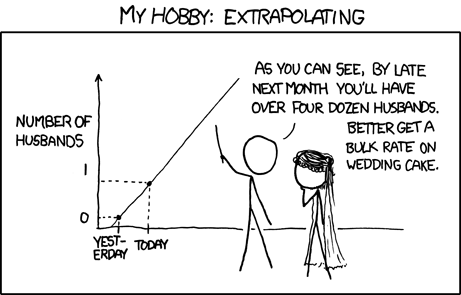
\includegraphics[width=10cm]{extrapolating.png}}
\end{figure}
\end{comment}


\begin{figure}[h!]
% \floatbox[{\capbeside\thisfloatsetup{capbesideposition={right,bottom},capbesidewidth=4cm}}]{figure}[\FBwidth]
% {\caption*{Randall Munroe, xkcd}}
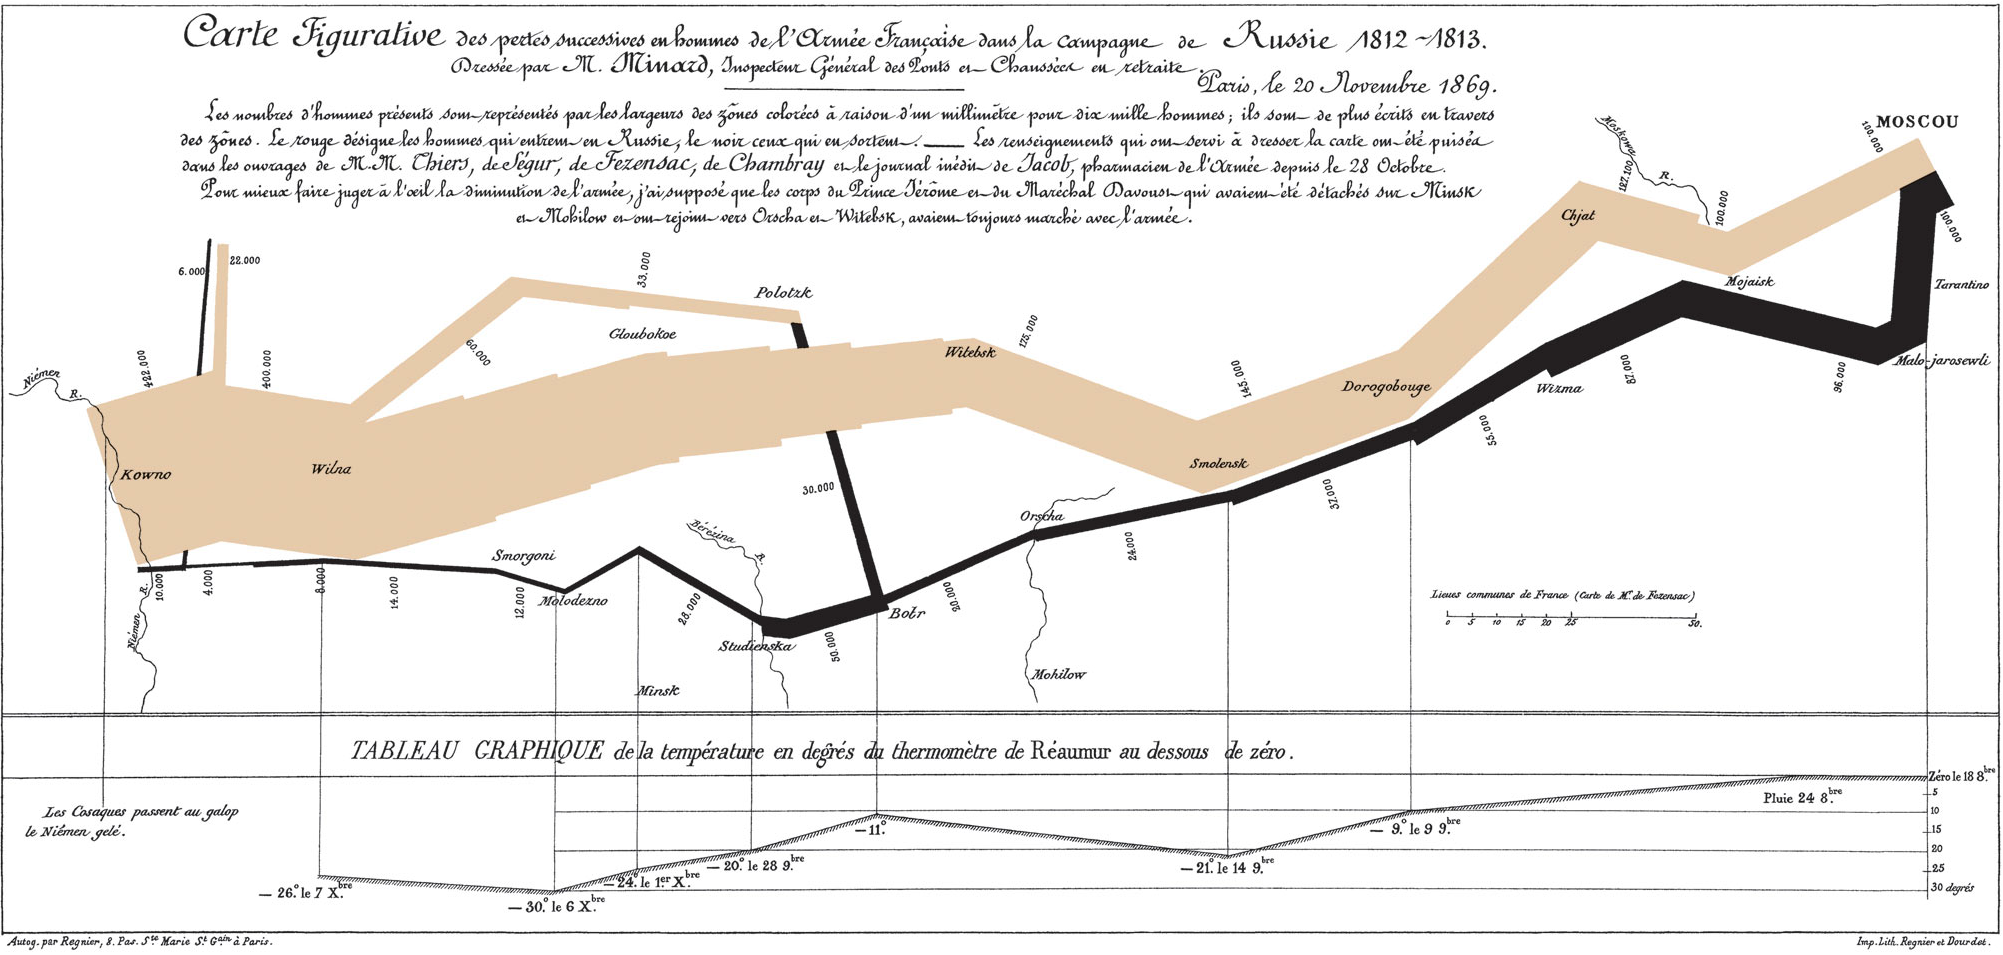
\includegraphics[width=19cm]{Minard.png}
\caption*{Charles Joseph Minard, Схема потерь наполеоновской армии в компании 1812-1813 годов}
\end{figure}




\end{document}
